  \cite{BufferStockTheory} derives an upper limit  $\MPCmax_{t}$ for the MPC as $m_{t}$
  approaches its lower bound.  Using this
  fact plus the strict concavity of the consumption function yields the
  proposition that
  \begin{equation}\begin{gathered}\begin{aligned}
        \cFunc_{t}(\ushort{m}_{t}+\aboveMin \mNrm_{t}) & < \MPCmax_{t} \aboveMin \mNrm_{t}.
      \end{aligned}\end{gathered}\end{equation}

  The solution method described above does not guarantee that
  approximated consumption will respect this constraint between gridpoints, and a failure to
  respect the constraint can occasionally cause computational problems in solving
  or simulating the model.  Here, we
  describe a method for constructing an approximation that always
  satisfies the constraint.

  \begin{comment} % Old text needs to be revised or eliminated
    That is, the realist's consumption function is bounded from above by both
    the \textit{unconstrained} optimist's problem already treated, as well as
    by the \textit{constrained} optimist's problem, which is a 45 degree line
    originating from $\ushort{m}_{t}$ on the $m$-axis, as shown in
    Figure~\ref{fig:IntExpFOCInvPesReaOptNeed45Plot}. The same is true for
    the value function, as illustrated in Figure
    \ref{fig:IntExpFOCInvPesReaOptNeed45ValuePlot}.

    \hypertarget{IntExpFOCInvPesReaOptNeed45Plot}{}
    \begin{figure}
      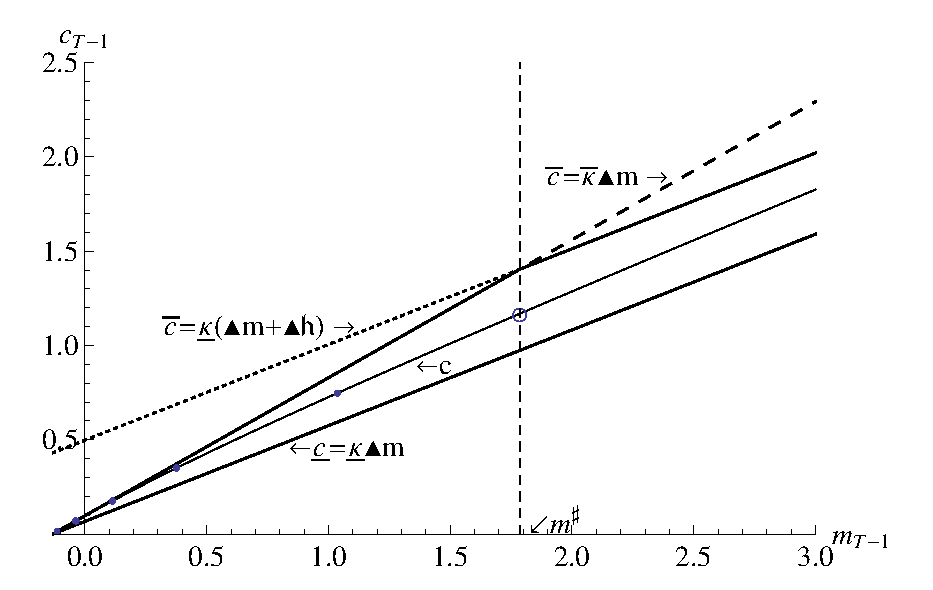
\includegraphics[width=6in]{./Figures/IntExpFOCInvPesReaOptNeed45Plot}
      \caption{45 Degree Line as Another Upper Bound}
      \label{fig:IntExpFOCInvPesReaOptNeed45Plot}
    \end{figure}

    \hypertarget{IntExpFOCInvPesReaOptNeed45ValuePlot}{}
    \begin{figure}
      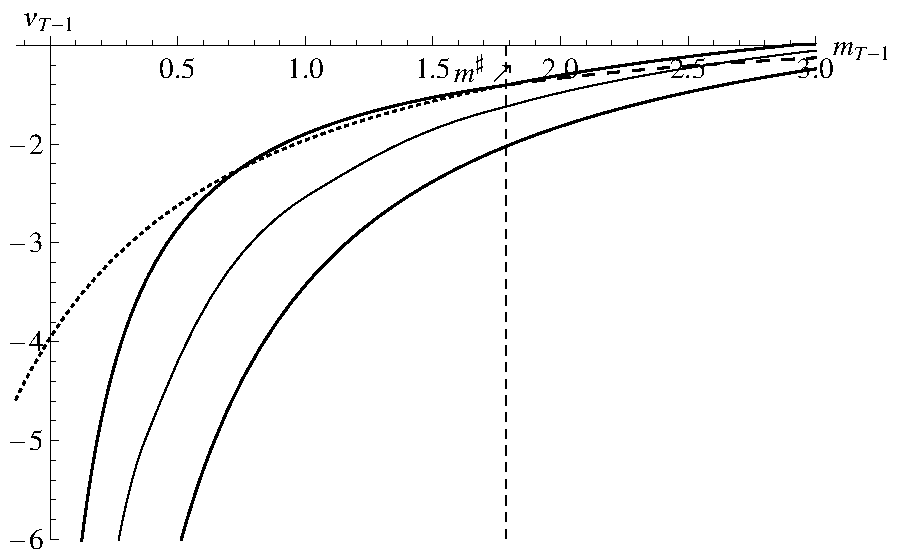
\includegraphics[width=6in]{./Figures/IntExpFOCInvPesReaOptNeed45ValuePlot}
      \caption{A Constrained Optimist's Value Function as Another Upper Bound}
      \label{fig:IntExpFOCInvPesReaOptNeed45ValuePlot}
    \end{figure}

  \end{comment}

  \newcommand{\mtCusp}{\ensuremath{\mNrm_{t}^{\#}}}
  % \newcommand{\aboveMin \mtCusp}{\ensuremath{\aboveMin \mNrm_{t}^{\#}}}
